%% LaTeX2e class for seminar theses
%% sections/content.tex
%% 
%% Karlsruhe Institute of Technology
%% Institute for Program Structures and Data Organization
%% Chair for Software Design and Quality (SDQ)
%%
%% Dr.-Ing. Erik Burger
%% burger@kit.edu
%%
%% Version 1.0, 2018-04-16

\section{Basics}
\label{ch:Basics}

First of all the basics of Bitcoin are needed to know what exactly was changed. \todo{maybe a bit longer}

\subsection{Transaction}
\label{sec:Introduction:Basics:Transaction}

\begin{figure}[!ht]
    \centering
    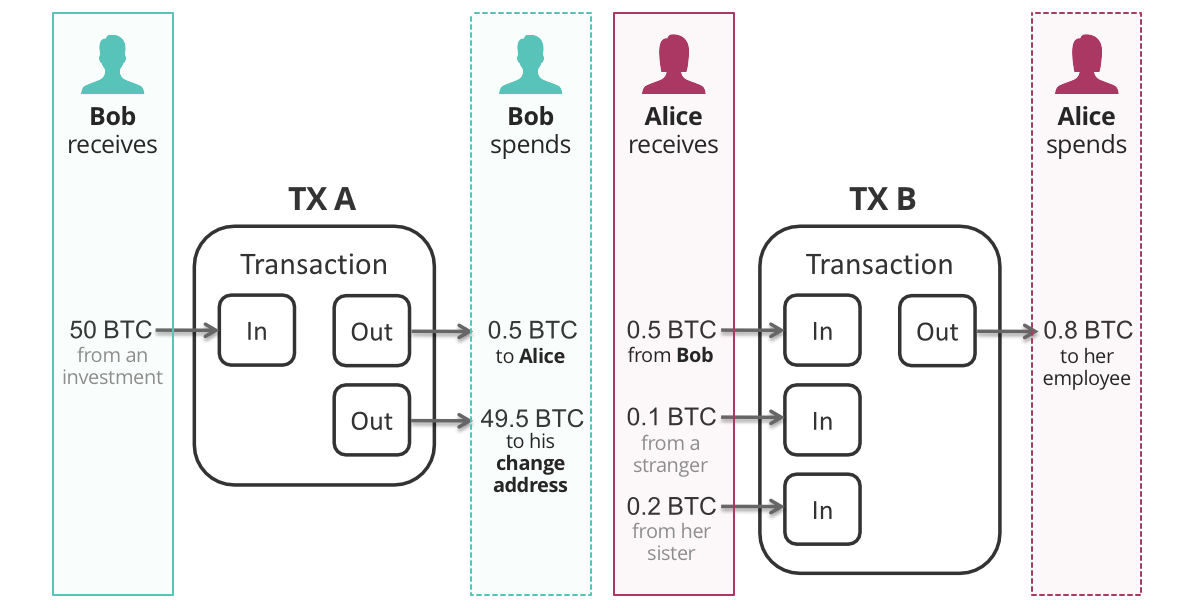
\includegraphics[width=\textwidth]{Ausarbeitung/images/transaction.png} \caption[Transaction]{Transaction\textsuperscript{1}} \small\textsuperscript{1} \url{https://thecoinrise.com/wp-content/uploads/2019/08/how-do-bitcoin-transaction-work.png}
    \label{fig:transaction}
\end{figure}
Transaction is built up with a version number, transaction inputs, transaction outputs and a lock time. \\
The version number just defines which version is used in this transaction. This can be differently for different transactions. \\
The lock time describes when the transaction should be seen as final. Either it is empty and it should be seen as final on publication, or it has a block height or timestamp as an argument, which tells when the transaction is final. \\
The first transaction in any block is called "coinbase" transaction and just credits a fix amount of bitcoins plus the sum of all transaction fees in the block. The transaction fees aggregate when the inputs of a transaction contain more bitcoin than the outputs. \\
Every transaction in any block must have at least one input and at least one output. The inputs must, except in the "coinbase" transaction, refer to an output of a previous transaction which was not spent yet, called an unspent transaction output or UTXO. For example the first input of Tx B in \autoref{fig:transaction} refers to the first output of Tx A, which is just spent in Tx B \\
Finally the transaction has to be signed. There are multiple ways to do this, but the signature is always, before SegWit, contained inside of a transaction.


\subsection{Merkle Tree}
\begin{figure}[!ht]
    \centering
    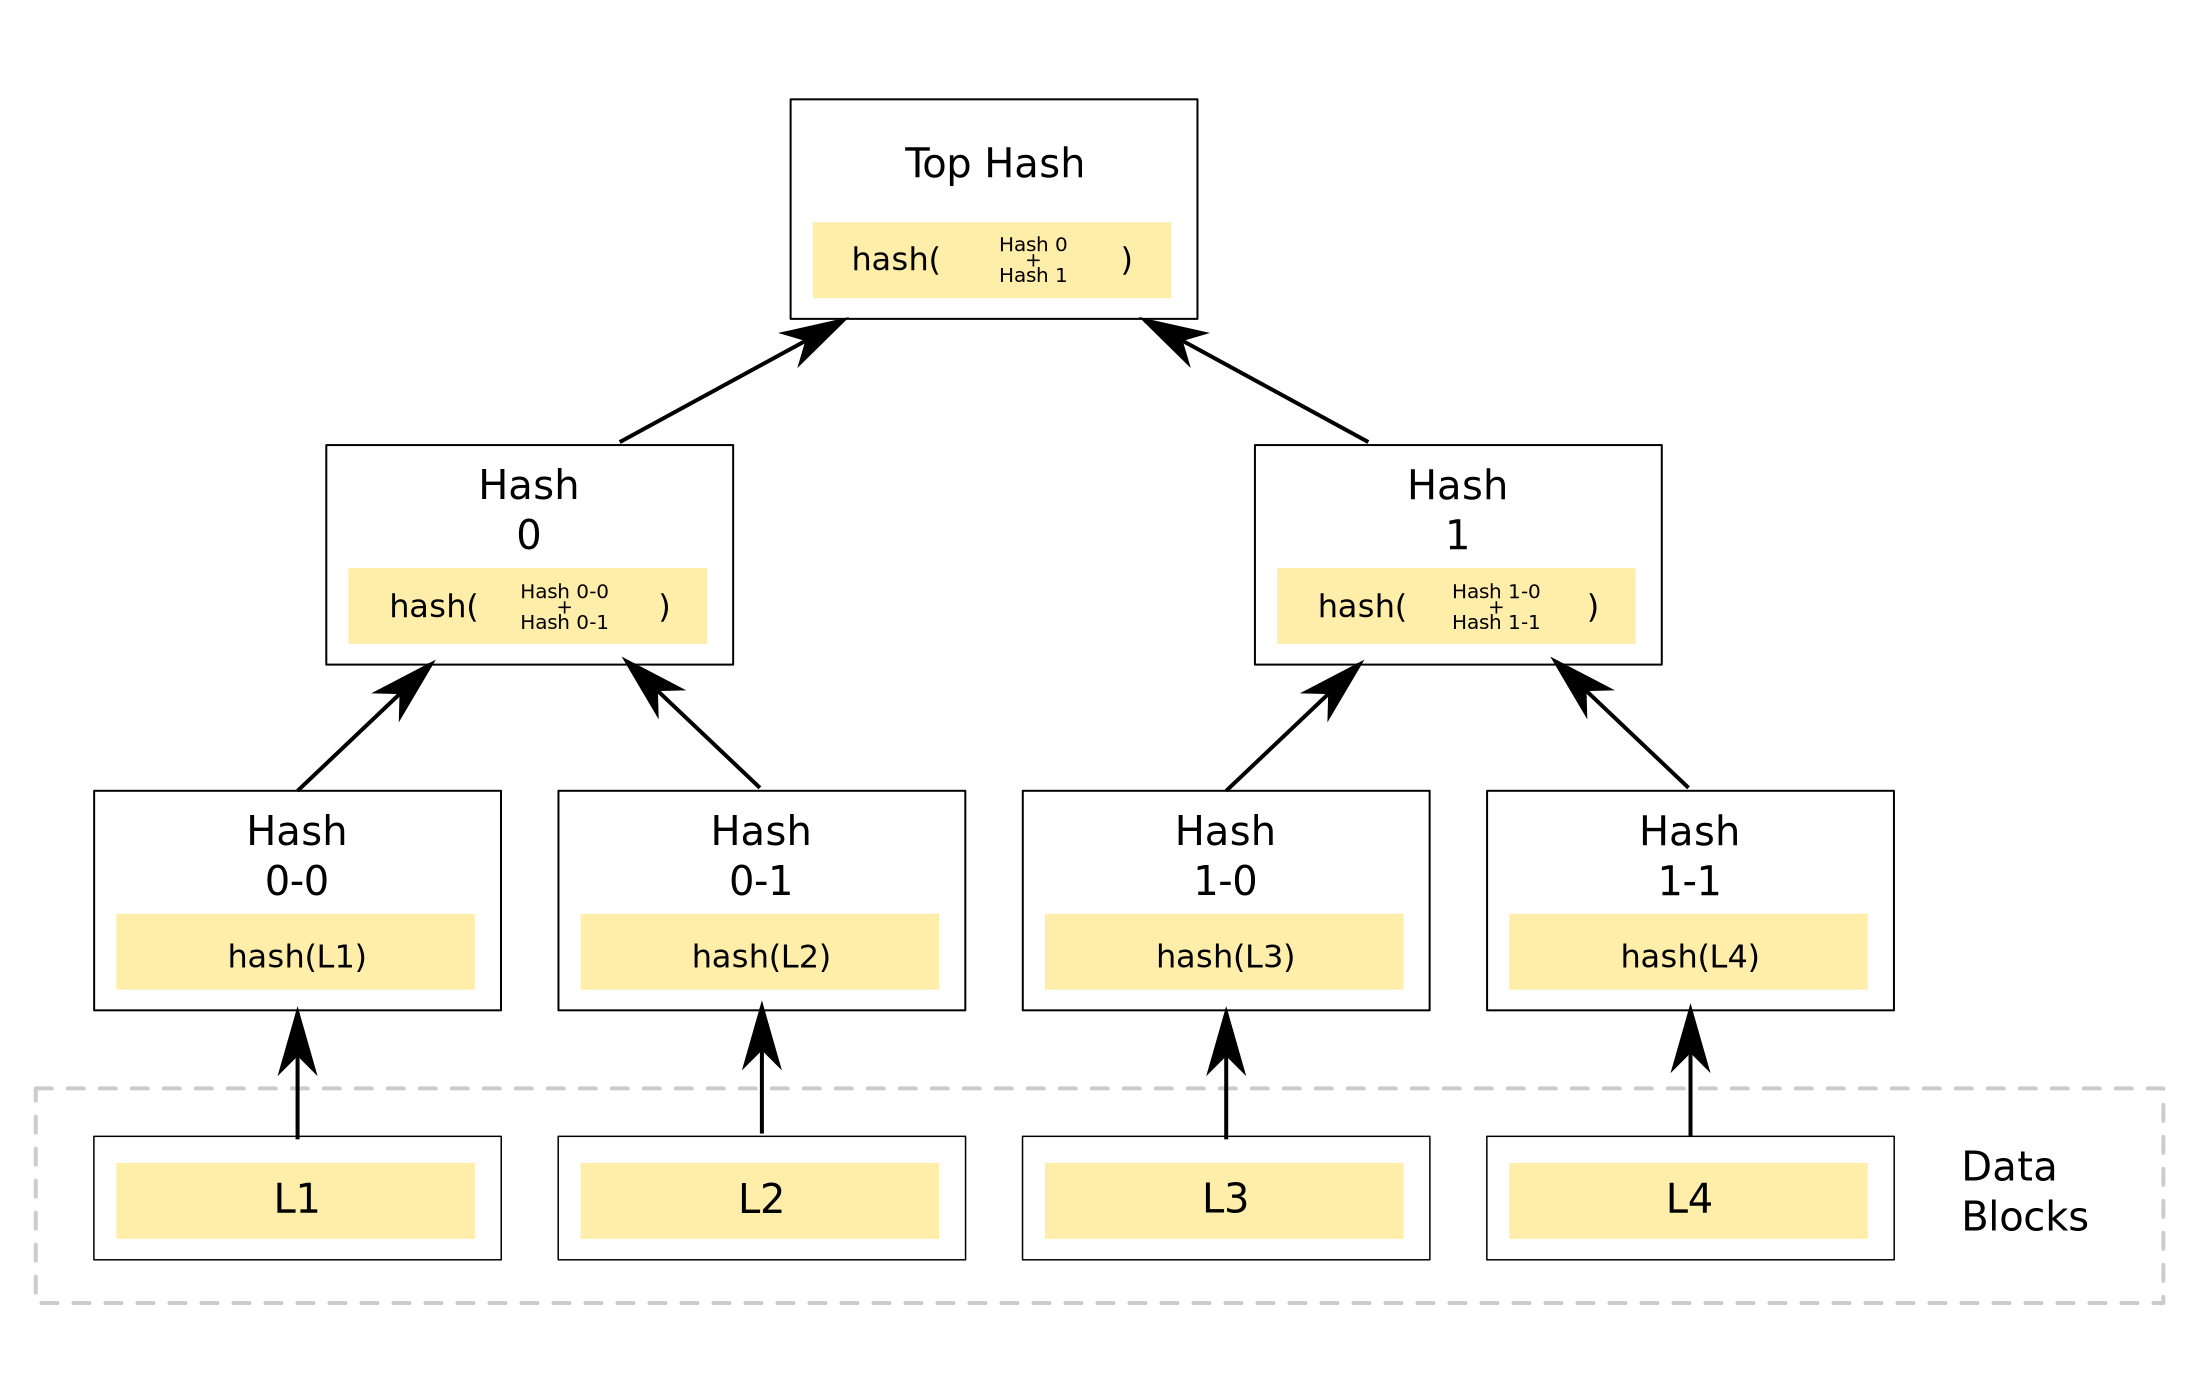
\includegraphics[width=(\textwidth * 2 / 3 )]{Ausarbeitung/images/merkle_tree.png}
    \caption[Merkle Tree]{Merkle Tree\textsuperscript{2}}
    \small\textsuperscript{2} \url{https://www.researchgate.net/figure/An-example-of-Merkle-Tree_fig1_327601654} 
    \label{fig:merkle_tree}
\end{figure}
A merkle tree, or binary hash tree as shown in \autoref{fig:merkle_tree}, is a tree, where all the leaves, in the case of bitcoin the leaves are the transactions of a block, are concatenated and then hashed pairwise. This results in a new layer of nodes, which are then again concatenated and then hashed pairwise until there is only one node left, called the merkle root. The merkle root would then in \autoref{fig:merkle_tree} be the "Top Hash", while 


\subsection{Blocksize limit}
\label{sec:Basics:BlocksizeLimit}

\todo{limitation to 1MB blocks limiting number of transactions per second to 4, compare to visa, \dots}



\subsection{Transaction Malleability}
\label{ch:TransactionMalleability}

\todo{short description with example, attack on Mt.Gox to get perspective, maybe with subsubsections}



\section{Segregated Witness}
\label{ch:SegWit}

\todo{description of what segwit is}

\subsection{Idee}
\label{sec:SegWit:Idee}

\todo{describe idea of moving witness to extra data structure}


\subsection{Implementation}
\label{sec:SegWit:Implementierung}

\todo{changes to transaction ID, witness programs functionality and script semantics, other consensus critical limits, additional definitions, commitment structure, extensible commitment structure, Backward compatibility}

\subsection{Consequences}
\label{sec:SegWit:Consequences}

\todo{Fixes transaction malleability, increases blocksize limit to an extent -> no solution but rather a slight improvement}

\subsection{Future possibilities}
\label{sec:SegWit:Future}
\todo{Trust-free unconfirmed transaction dependency chain (Lightning Network), Future extensions}

\subsection{History of Segregated Witness}
\label{sec:SegWit:History}

\todo{find good source for this}

%\subsection{Trial of SegWit2x}